The parameters are then listed in  
    \tabref{tab:chapters/11/11/5/3/points}.
\begin{table}[H]
	\centering
    %%%%%%%%%%%%%%%%%%%%%%%%%%%%%%%%%%%%%%%%%%%%%%%%%%%%%%%%%%%%%%%%%%%%%%
%%                                                                  %%
%%  This is the header of a LaTeX2e file exported from Gnumeric.    %%
%%                                                                  %%
%%  This file can be compiled as it stands or included in another   %%
%%  LaTeX document. The table is based on the longtable package so  %%
%%  the longtable options (headers, footers...) can be set in the   %%
%%  preamble section below (see PRAMBLE).                           %%
%%                                                                  %%
%%  To include the file in another, the following two lines must be %%
%%  in the including file:                                          %%
%%        \def\inputGnumericTable{}                                 %%
%%  at the beginning of the file and:                               %%
%%        \input{name-of-this-file.tex}                             %%
%%  where the table is to be placed. Note also that the including   %%
%%  file must use the following packages for the table to be        %%
%%  rendered correctly:                                             %%
%%    \usepackage[latin1]{inputenc}                                 %%
%%    \usepackage{color}                                            %%
%%    \usepackage{array}                                            %%
%%    \usepackage{longtable}                                        %%
%%    \usepackage{calc}                                             %%
%%    \usepackage{multirow}                                         %%
%%    \usepackage{hhline}                                           %%
%%    \usepackage{ifthen}                                           %%
%%  optionally (for landscape tables embedded in another document): %%
%%    \usepackage{lscape}                                           %%
%%                                                                  %%
%%%%%%%%%%%%%%%%%%%%%%%%%%%%%%%%%%%%%%%%%%%%%%%%%%%%%%%%%%%%%%%%%%%%%%



%%  This section checks if we are begin input into another file or  %%
%%  the file will be compiled alone. First use a macro taken from   %%
%%  the TeXbook ex 7.7 (suggestion of Han-Wen Nienhuys).            %%
\def\ifundefined#1{\expandafter\ifx\csname#1\endcsname\relax}


%%  Check for the \def token for inputed files. If it is not        %%
%%  defined, the file will be processed as a standalone and the     %%
%%  preamble will be used.                                          %%
\ifundefined{inputGnumericTable}

%%  We must be able to close or not the document at the end.        %%
	\def\gnumericTableEnd{\end{document}}


%%%%%%%%%%%%%%%%%%%%%%%%%%%%%%%%%%%%%%%%%%%%%%%%%%%%%%%%%%%%%%%%%%%%%%
%%                                                                  %%
%%  This is the PREAMBLE. Change these values to get the right      %%
%%  paper size and other niceties.                                  %%
%%                                                                  %%
%%%%%%%%%%%%%%%%%%%%%%%%%%%%%%%%%%%%%%%%%%%%%%%%%%%%%%%%%%%%%%%%%%%%%%

	\documentclass[12pt%
			  %,landscape%
                    ]{report}
       
\begin{document}


%%  End of the preamble for the standalone. The next section is for %%
%%  documents which are included into other LaTeX2e files.          %%
\else

%%  We are not a stand alone document. For a regular table, we will %%
%%  have no preamble and only define the closing to mean nothing.   %%
\def\gnumericTableEnd{}

%%  If we want landscape mode in an embedded document, comment out  %%
%%  the line above and uncomment the two below. The table will      %%
%%  begin on a new page and run in landscape mode.                  %%
%       \def\gnumericTableEnd{\end{landscape}}
%       \begin{landscape}


%%  End of the else clause for this file being \input.              %%
\fi

%%%%%%%%%%%%%%%%%%%%%%%%%%%%%%%%%%%%%%%%%%%%%%%%%%%%%%%%%%%%%%%%%%%%%%
%%                                                                  %%
%%  The rest is the gnumeric table, except for the closing          %%
%%  statement. Changes below will alter the table's appearance.     %%
%%                                                                  %%
%%%%%%%%%%%%%%%%%%%%%%%%%%%%%%%%%%%%%%%%%%%%%%%%%%%%%%%%%%%%%%%%%%%%%%

\providecommand{\gnumericmathit}[1]{#1}
%%  Uncomment the next line if you would like your numbers to be in %%
%%  italics if they are italizised in the gnumeric table.           %%
%\renewcommand{\gnumericmathit}[1]{\mathit{#1}}
\providecommand{\gnumericPB}[1]%
{\let\gnumericTemp=\\#1\let\\=\gnumericTemp\hspace{0pt}}
\ifundefined{gnumericTableWidthDefined}
\newlength{\gnumericTableWidth}
\newlength{\gnumericTableWidthComplete}
\newlength{\gnumericMultiRowLength}
\global\def\gnumericTableWidthDefined{}
\fi
%% The following setting protects this code from babel shorthands.  %%
\ifthenelse{\isundefined{\languageshorthands}}{}{\languageshorthands{english}}
%%  The default table format retains the relative column widths of  %%
%%  gnumeric. They can easily be changed to c, r or l. In that case %%
%%  you may want to comment out the next line and uncomment the one %%
%%  thereafter                                                      %%
\providecommand\gnumbox{\makebox[0pt]}
%%\providecommand\gnumbox[1][]{\makebox}

%% to adjust positions in multirow situations                       %%
\setlength{\bigstrutjot}{\jot}
\setlength{\extrarowheight}{\doublerulesep}

%%  The \setlongtables command keeps column widths the same across  %%
%%  pages. Simply comment out next line for varying column widths.  %%
\setlongtables

\setlength\gnumericTableWidth{%
       53pt+%
       171pt+%
       53pt+%
       0pt}
\def\gumericNumCols{3}
\setlength\gnumericTableWidthComplete{\gnumericTableWidth+%
       \tabcolsep*\gumericNumCols*2+\arrayrulewidth*\gumericNumCols}
\ifthenelse{\lengthtest{\gnumericTableWidthComplete > \linewidth}}%
{\def\gnumericScale{1*\ratio{\linewidth-%
                     \tabcolsep*\gumericNumCols*2-%
                     \arrayrulewidth*\gumericNumCols}%
              {\gnumericTableWidth}}}%
{\def\gnumericScale{1}}

%%%%%%%%%%%%%%%%%%%%%%%%%%%%%%%%%%%%%%%%%%%%%%%%%%%%%%%%%%%%%%%%%%%%%%
%%                                                                  %%
%% The following are the widths of the various columns. We are      %%
%% defining them here because then they are easier to change.       %%
%% Depending on the cell formats we may use them more than once.    %%
%%                                                                  %%
%%%%%%%%%%%%%%%%%%%%%%%%%%%%%%%%%%%%%%%%%%%%%%%%%%%%%%%%%%%%%%%%%%%%%%

\ifthenelse{\isundefined{\gnumericColA}}{\newlength{\gnumericColA}}{}\settowidth{\gnumericColA}{\begin{tabular}{@{}p{40pt*\gnumericScale}@{}}x\end{tabular}}
\ifthenelse{\isundefined{\gnumericColB}}{\newlength{\gnumericColB}}{}\settowidth{\gnumericColB}{\begin{tabular}{@{}p{171pt*\gnumericScale}@{}}x\end{tabular}}
\ifthenelse{\isundefined{\gnumericColC}}{\newlength{\gnumericColC}}{}\settowidth{\gnumericColC}{\begin{tabular}{@{}p{60pt*\gnumericScale}@{}}x\end{tabular}}

\begin{tabular}[c]{%
              b{\gnumericColA}%
              b{\gnumericColB}%
              b{\gnumericColC}%
       }

       %%%%%%%%%%%%%%%%%%%%%%%%%%%%%%%%%%%%%%%%%%%%%%%%%%%%%%%%%%%%%%%%%%%%%%
       %%  The longtable options. (Caption, headers... see Goosens, p.124) %%
       %	\caption{The Table Caption.}             \\	%
       % \hline	% Across the top of the table.
       %%  The rest of these options are table rows which are placed on    %%
       %%  the first, last or every page. Use \multicolumn if you want.    %%

       %%  Header for the first page.                                      %%
       %	\multicolumn{3}{c}{The First Header} \\ \hline 
       %	\multicolumn{1}{c}{colTag}	%Column 1
       %	&\multicolumn{1}{c}{colTag}	%Column 2
       %	&\multicolumn{1}{c}{colTag}	\\ \hline %Last column
       %	\endfirsthead

       %%  The running header definition.                                  %%
       %	\hline
       %	\multicolumn{3}{l}{\ldots\small\slshape continued} \\ \hline
       %	\multicolumn{1}{c}{colTag}	%Column 1
       %	&\multicolumn{1}{c}{colTag}	%Column 2
       %	&\multicolumn{1}{c}{colTag}	\\ \hline %Last column
       %	\endhead

       %%  The running footer definition.                                  %%
       %	\hline
       %	\multicolumn{3}{r}{\small\slshape continued\ldots} \\
       %	\endfoot

       %%  The ending footer definition.                                   %%
       %	\multicolumn{3}{c}{That's all folks} \\ \hline 
       %	\endlastfoot
       %%%%%%%%%%%%%%%%%%%%%%%%%%%%%%%%%%%%%%%%%%%%%%%%%%%%%%%%%%%%%%%%%%%%%%

       \hhline{|-|-|-}
       \multicolumn{1}{|p{\gnumericColA}|}%
	{\gnumericPB {\centering}$\vec{O}$}
        & \multicolumn{1}{p{\gnumericColB}|} %
       {\gnumericPB{\raggedright}\gnumbox[l]{Lowest point of cable}}
        & \multicolumn{1}{p{\gnumericColC}|} %
       {\gnumericPB{\raggedright}\gnumbox[l]{\myvec{0 \\ 0}}}
       \\
       \hhline{|-|-|-|}
       \multicolumn{1}{|p{\gnumericColA}|}%
       {\gnumericPB{\raggedright}\gnumbox[l]{$d$}}
        & \multicolumn{1}{p{\gnumericColB}|} %
       {\gnumericPB{\raggedright}\gnumbox[l]{Length of the cable}}
        & \multicolumn{1}{p{\gnumericColC}|} %
       {\gnumericPB{\raggedright}\gnumbox[l]{100 m}}
       \\
       \hhline{|-|-|-|}
       \multicolumn{1}{|p{\gnumericColA}|}%
       {\gnumericPB{\raggedright}\gnumbox[l]{$d_1$}}
        & \multicolumn{1}{p{\gnumericColB}|} %
       {\gnumericPB{\raggedright}\gnumbox[l]{Length of longest wire}}
        & \multicolumn{1}{p{\gnumericColC}|} %
       {\gnumericPB{\raggedright}\gnumbox[l]{30 m}}
       \\
       \hhline{|-|-|-|}
       \multicolumn{1}{|p{\gnumericColA}|}%
       {\gnumericPB{\raggedright}\gnumbox[l]{$d_2$}}
        & \multicolumn{1}{p{\gnumericColB}|} %
       {\gnumericPB{\raggedright}\gnumbox[l]{Length of shortest wire}}
        & \multicolumn{1}{p{\gnumericColC}|} %
       {\gnumericPB{\raggedright}\gnumbox[l]{6 m}}
       \\
       \hhline{|-|-|-|}
       \multicolumn{1}{|p{\gnumericColA}|}%
       {\gnumericPB{\raggedright}$\vec{A}$}
        & \multicolumn{1}{p{\gnumericColB}|} %
       {\gnumericPB{\raggedright}\gnumbox[l]{End point of cable}}
        & \multicolumn{1}{p{\gnumericColC}|} %
       {\gnumericPB{\raggedright}\gnumbox[l]{\myvec{\frac{d}{2}\\d_1-d_2}}}
       \\
       \hhline{|-|-|-|}
       \multicolumn{1}{|p{\gnumericColA}|}%
       {\gnumericPB{\raggedright}$\vec{B}$}
        & \multicolumn{1}{p{\gnumericColB}|} %
       {\gnumericPB{\raggedright}\gnumbox[l]{End point of cable}}
        & \multicolumn{1}{p{\gnumericColC}|} %
       {\gnumericPB{\raggedright}\gnumbox[l]{\myvec{-\frac{d}{2}\\d_1-d_2}}}
       \\
       \hhline{|-|-|-|}

\end{tabular}

\ifthenelse{\isundefined{\languageshorthands}}{}{\languageshorthands{\languagename}}
\gnumericTableEnd
    \caption{points}
    \label{tab:chapters/11/11/5/3/points}
\end{table}
For the conic,
\begin{align}
    \vec{V} = \myvec{1&0\\0&0}.
\end{align}
Points $\vec{O}, \vec{A}$, and $\vec{B}$ are on conic, so we have
\begin{align}
	\vec{O}^{\top}\vec{V}\vec{O} + 2\vec{u}^{\top}\vec{O} + f &= 0\\
	\vec{A}^{\top}\vec{V}\vec{A} + 2\vec{u}^{\top}\vec{A} + f &= 0\\
	\vec{B}^{\top}\vec{V}\vec{B} + 2\vec{u}^{\top}\vec{B} + f &= 0	 
\end{align}
which can be expressed as
\begin{align}
	2\vec{O}^{\top}\vec{u} + f &= - \vec{O}^{\top}\vec{V}\vec{O}\\
	2\vec{A}^{\top}\vec{u} + f &= - \vec{A}^{\top}\vec{V}\vec{A}\\
	2\vec{B}^{\top}\vec{u} + f &= - \vec{B}^{\top}\vec{V}\vec{B}	
\end{align}
leading to the matrix equation
\begin{align}
	\myvec{2\vec{O}^{\top} & 1\\ 2\vec{A}^{\top} & 1\\ 2\vec{B}^{\top} & 1}\myvec{\vec{u} \\ f} = -\myvec{\vec{O}^{\top}\vec{V}\vec{O}\\ \vec{A}^{\top}\vec{V}\vec{A}\\ \vec{B}^{\top}\vec{V}\vec{B}}
\end{align}
Substituting numerical values in the above equation,
\begin{align}
    \myvec{0&0&1\\ 100&48&1\\ -100&48&1}\myvec{\vec{u} \\ f} = -\myvec{0\\-2500\\-2500}\\
    \implies f = 0 \text{ and } \vec{u} = \myvec{0\\-\frac{625}{12}}
\end{align}
So, the equation of the parabola is
\begin{align}
    \label{eq:chapters/11/11/5/3/parab1}  \vec{x}^{\top}\myvec{1&0\\0&0}\vec{x} + 2\myvec{0&-\frac{625}{12}}\vec{x} = 0 
\end{align}
The desired point can be expressed as
\begin{align}
	\vec{D} = \myvec{18 \\ x_2}
\end{align}
Substituting this in the parabola equation,
\begin{align}
    18^2 - \frac{6}{625}\lambda_2 = 0
    \\
\implies \lambda_2 = \frac{1944}{625}
\end{align}
Thus, the length of a supporting wire attached to the roadway $18 m$ from the middle is 
\begin{align}
     \lambda_2 + d_2 = \frac{5694}{625} m   
\end{align}
See  
    \figref{fig:chapters/11/11/5/3/parabola}.
\begin{figure}[H]
    \centering
    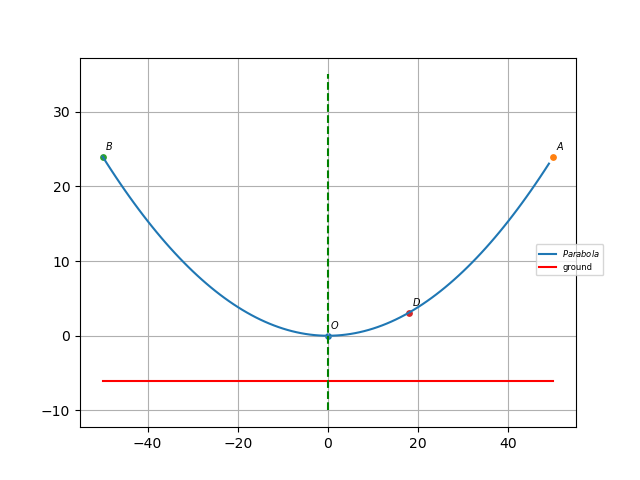
\includegraphics[width=0.75\columnwidth]{chapters/11/11/5/3/figs/parabola.png}
    \caption{}
    \label{fig:chapters/11/11/5/3/parabola}
\end{figure}

